\documentclass[12pt, letterpaper, titlepage]{article}
\usepackage[utf8]{inputenc}
\usepackage{geometry}
\usepackage{color,graphicx,overpic,colortbl} 
\usepackage{fancyhdr}
\usepackage{amsmath,amsthm,amsfonts,amssymb}
\usepackage{mathtools}
\usepackage{hyperref}
\usepackage{multicol}
\usepackage{array}
\usepackage{float}
\usepackage{blindtext}
\usepackage{longtable}
\usepackage{scrextend}
\usepackage[font=small,labelfont=bf]{caption}
\usepackage{calc}
\usepackage{titlesec}
\usepackage{listings}
\usepackage[normalem]{ulem}
\usepackage{tabularx}
\usepackage{mathrsfs}
\usepackage{bookmark}
\usepackage{apple_emoji}
\usepackage{setspace}
\usepackage{ragged2e}
\usepackage{ltablex}
\usepackage{xurl}
\usepackage{tikz}
\usepackage{pgfplots}

\mathtoolsset{showonlyrefs}  
\allowdisplaybreaks

\newcolumntype{q}{>{\hsize=.45\hsize}X}
\newcolumntype{s}{>{\hsize=.15\hsize}X}

\definecolor{mycolor}{rgb}{0, 0, 0}

\geometry{top=2.54cm, left=2.54cm, right=2.54cm, bottom=2.54cm}
\setlength{\headheight}{20pt}
\setlength{\parskip}{0.5cm}
\setlength{\parindent}{1cm}

\pgfplotsset{width=\textwidth-3cm,compat=newest}
\usepgfplotslibrary{patchplots}
\renewcommand{\thesection}{} % Make sections have no number

\newcommand{\B}{
\includegraphics[height=1.5em, valign=B, raise=-0.2em]{BigB.png}} 
\newcommand{\nx}{$n\times1$}

\title{\textbf{\Huge{
    \begin{center}
        ECE 322 Lab Report \#2
    \end{center}
}}}
\author{
\B enjamin Kong \\
1573684 \\
}

\pagestyle{fancy}
\fancyhf{}
\rhead{\thepage}
\lhead{\textit{ECE 322 Lab Report \#2}}

\begin{document} 
\onehalfspacing

\maketitle
\newpage

\tableofcontents
\newpage

\section{Introduction}
The purpose of this lab was to introduce two testing techniques: extreme point combination (EPC) and weak \nx. 

EPC involves performing domain analysis for a given subdomain in order to find the domain limits for each dimension (input). For each limit found, we create test cases for slightly under the min, the min, the max, and slightly over the max. We then produce all possible combinations of these test cases. We also choose one set of inputs that is inside the valid subdomain. This should result in $4^n+1$ test cases where $n$ is the number of inputs. 

Weak \nx\ involves finding linear boundaries for the problem through domain analysis. For each boundary, we select $n$ boundaries where $n$ is the number of inputs along with one point located off the boundary. Since the boundaries are linear, each boundary can be fully specified with $n$ points. For the point that is located off the boundary: if the boundary is open, we choose a point within the boundary; otherwise, we choose a point outside the boundary. This should result in $b(n+1)+1$ test cases where $b$ is the number of linear boundaries.

\section{Part 1 | Drone Program}
\subsection*{Q1}
In part 1, we tested the Drone program using EPC and weak \nx\ testing techniques. The Drone program is a command-line program written in Java. It takes three inputs: $x_1$, $x_2$, and $x_3$ which must all be positive integers. The Drone program should output ``Success!'' if $x_1 + x_2 + x_3 \leq k$ where $k=100$ for this lab. Otherwise, the program should output ``Failure!'' If the inputs are not all positive integers, the program should output ``ERROR: Invalid argument - negative value.''

\subsection*{Q2}
For the EPC tests, it we found 9 failed test cases. All of these failed cases involved $x_2$ being a negative integer. We expect that the program should output the error message; however, the program outputs the success or failure message. This is likely because the program doesn't check if $x_2$ satisfies $x_2\geq0$.

For the weak \nx\ tests, we found a failed test case just outside of the $x_2=0$ boundary. We expect the error message for a negative input, but instead we get the success message. This is again likely because the program doesn't check if $x_2$ satisfies $x_2\geq0$.

\subsection*{Q3}
\begin{figure}[H]
\centering
\caption{Subdomain of valid inputs for Drone program.}
\begin{tikzpicture}

\begin{axis} [
    view = {65}{25},
    xmin = 0,
    xmax = 100,
    ymin = 0,
    ymax = 100,
    zmin = 0,
    zmax = 100,
    xlabel = $x_1$,
    ylabel = $x_2$,
    zlabel = $x_3$,
    xtick = {0, 25, 50, 75, 100},
    ytick = {0, 25, 50, 75, 100},
    ztick = {0, 25, 50, 75, 100},
    grid,
    colormap/violet
]

\addplot3 [
    opacity = 0.5,
    table/row sep = \\,
    patch,
    patch type = polygon,
    faceted color = teal,
    vertex count = 3,
    patch table with point meta = {
        0 1 2 0 \\
        0 1 3 1 \\
        0 2 3 2 \\
        1 2 3 3 \\
    },
] table {
    x y z \\
    0 0 0 \\
    0 0 100 \\
    0 100 0 \\
    100 0 0 \\
};

\end{axis}

\end{tikzpicture}
\end{figure}

\subsection*{Q4}
The EPC testing found 9 failed test cases. Meanwhile, the weak \nx\ testing found 1 failed test case. We can be reasonably confident in saying that all the failed test cases stemmed from the same issue: that the Drone program doesn't check that $x_2>=0$. While the EPC testing found more failed test cases than the weak \nx\ testing, both test techniques were effective in finding an error within the Drone program. However, the weak \nx\ technique was more efficient here, requiring only 17 total test cases compared with 65 for the EPC technique.

\subsection*{Q5}
See the appendix for the tables (table 1 and table 2).

\section{Part 2 | Remote Car Program}
\subsection*{Q1}
In part 2, we tested the Remote Car program using EPC and weak \nx\ testing techniques. The Remote Car program is a command-line program written in Java. It takes two inputs $x$ and $y$ which represent coordinates on the Cartesian plane. If $(x,y)$ are inside a circle with radius $r = 1$ (centered about the origin), the program is expected to output ``Ok.'' Otherwise, it should output ``Out of range!'' The inputs $x$ and $y$ should be real numbers.

\subsection*{Q2}
For the weak \nx\ testing, we need to approximate the circle with linear equations since we require linear boundaries for this testing technique. As a result, we approximated the circle with four linear equations as listed below:
\begin{equation}
    y = \begin{cases}
        x + 1 & -1 \leq x \leq 0 \\
        x - 1 & 0 \leq x \leq 1 \\
        -x + 1 & 0 \leq x \leq 1 \\
        -x - 1 & -1 \leq x \leq 0. \\
    \end{cases}
\end{equation}

\subsection*{Q3}
For the EPC testing, we had $4^2+1=17$ total test cases since we had two input variables. We chose 
\begin{itemize}
    \item slightly under min: -1.1,
    \item min: -1,
    \item max: 1, and
    \item slightly over max: 1.1.
\end{itemize}
Using a python script, we automatically tested the program with all combinations of the values stated above. The table can be found in the appendix as table 3. No failed test cases were found for EPC testing. The EPC testing seemed effective for testing the circle subdomain as there were no failed test cases.

For the weak \nx\ testing, we used 4 boundary lines. Since we had two input variables, we had $4(2+1)+1=13$ test cases. The table of these test cases and their results can be found in the appendix as table 4. Four failed test cases were found from the testing. All of these failed test cases involved testing just outside the linear boundaries.

For a circle, subdomain approximation is not very effective. This is because if a test case is chosen right outside a linear boundary, it can still be within the actual subdomain's boundary. This explains the test cases where we expected an out of range error, but got an ``Ok.''|these were approximation errors, not real errors. The weak \nx\ testing does not seem very effective for testing this particular subdomain. While it is efficient (only 13 test cases), it isn't effective. The result is somewhat meaningless since testing outside the boundary will almost always fail since the linear approximation is quite inaccurate. Overall, we conclude that the EPC technique is more effective for the circular subdomain. 

Using more linear segments would improve the approximation since more line segments can more accurately represent a circular domain. Weak \nx\ testing requires $b(n+1)+1$ test cases where $b$ is the number of segments and $n$ is the number of input variables. Hence, if we used 8 linear segments for this approximation, we would have $8(2+1)+1=25$ test cases.

\subsection*{Q4}
See the appendix for the tables (table 3 and table 4).

\section{Conclusion}
In this lab, we were introduced to EPC and weak \nx\ testing techniques. EPC testing involves finding domain limits for each input by performing domain analysis for a given subdomain, creating test cases for slightly under the min, the min, the max, and slightly over the max, then producing all possible combinations of these test cases. EPC testing results in $4^n+1$ test cases where $n$ is the number of inputs. Weak \nx\ testing involves finding linear boundaries through domain analysis, choosing $n$ points (where $n$ is the number of inputs) on the boundary and 1 point off the boundary per boundary, and creating test cases from these. Weak \nx\ testing results in $b(n+1)+1$ test cases where $b$ is the number of boundaries and $n$ is the number of inputs.

In part 1, we tested a Drone program. Using EPC testing, we found 9 failed test cases. Using weak \nx\ testing, we found one failed test case. Both of these were attributed to the same error: the Drone program wasn't ensuring that $x_2$ satisfied $x_2\geq0$.

In part 2, we tested a Remote Car program. Using EPC testing, we found no failed test cases. Using weak \nx\ testing, we found four failed test cases. However, we concluded that these failed cases were a result of a bad approximation and that these failed test cases were essentially meaningless in determining if the program worked correctly or not. 

We found that EPC worked well overall. In part 1, it allowed us to find a bug with the checking of $x_2$. In part 2, it helped make the case that the Remote Car program was working correctly. While EPC testing typically results in more test cases than weak \nx\ testing, it can be more effective in certain cases such as in part 2. In general, EPC is quite effective while also being quite efficient compared to other testing methods.

We found that the weak \nx\ testing worked decently overall. In part 1, it allowed us to find a bug with the checking of $x_2$ with only 17 test cases, which is more efficient than the EPC testing. However, for part 2, the weak \nx\ testing struggled as linear approximations don't work well in many cases such as this one. While the weak \nx\ testing struggled for the circular subdomain, it is typically quite effective and very efficient in regards to reducing the number of test cases.

Both EPC and weak \nx\ testing techniques usually require more work to set up the test cases than, say, error guessing. EPC testing requires more work because we need to perform domain analysis for the inputs. Furthermore, if the inputs are unbounded, it can be difficult to perform EPC in a meaningful way. For weak \nx\ testing, it can also be difficult to create test cases in some scenarios. For example, for part 2 with the Remote Car program, it is very difficult to approximate a circle using linear boundaries. Using more boundaries increases accuracy, but scales up the work proportional to the number of boundaries used.

\newpage

\section{Appendix}
\begin{tabularx}{\textwidth}{|q|q|s|s|s|X|X|}
    \caption{EPC test cases for Drone program.} \\
    \hline
    \textbf{TestID} & \textbf{Desc.} & $x_1$ & $x_2$ & $x_3$ & \textbf{Expected} & \textbf{Actual} \\
    \hline
    1 & EPC case & 0 & 0 & 0 & Success! & Success! \\
    \hline
    2 & EPC case & 0 & 0 & 100 & Success! & Success! \\
    \hline
    3 & EPC case & 0 & 0 & -1 & ERROR: Invald argument - negative value & ERROR: Invald argument - negative value \\
    \hline
    4 & EPC case & 0 & 0 & 101 & Failure! & Failure! \\
    \hline
    5 & EPC case & 0 & 100 & 0 & Success! & Success! \\
    \hline
    6 & EPC case & 0 & 100 & 100 & Failure! & Failure! \\
    \hline
    7 & EPC case & 0 & 100 & -1 & ERROR: Invald argument - negative value & ERROR: Invald argument - negative value \\
    \hline
    8 & EPC case & 0 & 100 & 101 & Failure! & Failure! \\
    \hline
    \rowcolor[HTML]{FFB9B9} 
    9 & EPC case & 0 & -1 & 0 & ERROR: Invald argument - negative value & Success! \\
    \hline
    \rowcolor[HTML]{FFB9B9} 
    10 & EPC case & 0 & -1 & 100 & ERROR: Invald argument - negative value & Success! \\
    \hline
    11 & EPC case & 0 & -1 & -1 & ERROR: Invald argument - negative value & ERROR: Invald argument - negative value \\
    \hline
    \rowcolor[HTML]{FFB9B9} 
    12 & EPC case & 0 & -1 & 101 & ERROR: Invald argument - negative value & Success! \\
    \hline
    13 & EPC case & 0 & 101 & 0 & Failure! & Failure! \\
    \hline
    14 & EPC case & 0 & 101 & 100 & Failure! & Failure! \\
    \hline
    15 & EPC case & 0 & 101 & -1 & ERROR: Invald argument - negative value & ERROR: Invald argument - negative value \\
    \hline
    16 & EPC case & 0 & 101 & 101 & Failure! & Failure! \\
    \hline
    17 & EPC case & 100 & 0 & 0 & Success! & Success! \\
    \hline
    18 & EPC case & 100 & 0 & 100 & Failure! & Failure! \\
    \hline
    19 & EPC case & 100 & 0 & -1 & ERROR: Invald argument - negative value & ERROR: Invald argument - negative value \\
    \hline
    20 & EPC case & 100 & 0 & 101 & Failure! & Failure! \\
    \hline
    21 & EPC case & 100 & 100 & 0 & Failure! & Failure! \\
    \hline
    22 & EPC case & 100 & 100 & 100 & Failure! & Failure! \\
    \hline
    23 & EPC case & 100 & 100 & -1 & ERROR: Invald argument - negative value & ERROR: Invald argument - negative value \\
    \hline
    24 & EPC case & 100 & 100 & 101 & Failure! & Failure! \\
    \hline
    \rowcolor[HTML]{FFB9B9} 
    25 & EPC case & 100 & -1 & 0 & ERROR: Invald argument - negative value & Success! \\
    \hline
    \rowcolor[HTML]{FFB9B9} 
    26 & EPC case & 100 & -1 & 100 & ERROR: Invald argument - negative value & Failure! \\
    \hline
    27 & EPC case & 100 & -1 & -1 & ERROR: Invald argument - negative value & ERROR: Invald argument - negative value \\
    \hline
    \rowcolor[HTML]{FFB9B9} 
    28 & EPC case & 100 & -1 & 101 & ERROR: Invald argument - negative value & Failure! \\
    \hline
    29 & EPC case & 100 & 101 & 0 & Failure! & Failure! \\
    \hline
    30 & EPC case & 100 & 101 & 100 & Failure! & Failure! \\
    \hline
    31 & EPC case & 100 & 101 & -1 & ERROR: Invald argument - negative value & ERROR: Invald argument - negative value \\
    \hline
    32 & EPC case & 100 & 101 & 101 & Failure! & Failure! \\
    \hline
    33 & EPC case & -1 & 0 & 0 & ERROR: Invald argument - negative value & ERROR: Invald argument - negative value \\
    \hline
    34 & EPC case & -1 & 0 & 100 & ERROR: Invald argument - negative value & ERROR: Invald argument - negative value \\
    \hline
    35 & EPC case & -1 & 0 & -1 & ERROR: Invald argument - negative value & ERROR: Invald argument - negative value \\
    \hline
    36 & EPC case & -1 & 0 & 101 & ERROR: Invald argument - negative value & ERROR: Invald argument - negative value \\
    \hline
    37 & EPC case & -1 & 100 & 0 & ERROR: Invald argument - negative value & ERROR: Invald argument - negative value \\
    \hline
    38 & EPC case & -1 & 100 & 100 & ERROR: Invald argument - negative value & ERROR: Invald argument - negative value \\
    \hline
    39 & EPC case & -1 & 100 & -1 & ERROR: Invald argument - negative value & ERROR: Invald argument - negative value \\
    \hline
    40 & EPC case & -1 & 100 & 101 & ERROR: Invald argument - negative value & ERROR: Invald argument - negative value \\
    \hline
    41 & EPC case & -1 & -1 & 0 & ERROR: Invald argument - negative value & ERROR: Invald argument - negative value \\
    \hline
    42 & EPC case & -1 & -1 & 100 & ERROR: Invald argument - negative value & ERROR: Invald argument - negative value \\
    \hline
    43 & EPC case & -1 & -1 & -1 & ERROR: Invald argument - negative value & ERROR: Invald argument - negative value \\
    \hline
    44 & EPC case & -1 & -1 & 101 & ERROR: Invald argument - negative value & ERROR: Invald argument - negative value \\
    \hline
    45 & EPC case & -1 & 101 & 0 & ERROR: Invald argument - negative value & ERROR: Invald argument - negative value \\
    \hline
    46 & EPC case & -1 & 101 & 100 & ERROR: Invald argument - negative value & ERROR: Invald argument - negative value \\
    \hline
    47 & EPC case & -1 & 101 & -1 & ERROR: Invald argument - negative value & ERROR: Invald argument - negative value \\
    \hline
    48 & EPC case & -1 & 101 & 101 & ERROR: Invald argument - negative value & ERROR: Invald argument - negative value \\
    \hline
    49 & EPC case & 101 & 0 & 0 & Failure! & Failure! \\
    \hline
    50 & EPC case & 101 & 0 & 100 & Failure! & Failure! \\
    \hline
    51 & EPC case & 101 & 0 & -1 & ERROR: Invald argument - negative value & ERROR: Invald argument - negative value \\
    \hline
    52 & EPC case & 101 & 0 & 101 & Failure! & Failure! \\
    \hline
    53 & EPC case & 101 & 100 & 0 & Failure! & Failure! \\
    \hline
    54 & EPC case & 101 & 100 & 100 & Failure! & Failure! \\
    \hline
    55 & EPC case & 101 & 100 & -1 & ERROR: Invald argument - negative value & ERROR: Invald argument - negative value \\
    \hline
    56 & EPC case & 101 & 100 & 101 & Failure! & Failure! \\
    \hline
    \rowcolor[HTML]{FFB9B9} 
    57 & EPC case & 101 & -1 & 0 & ERROR: Invald argument - negative value & Success! \\
    \hline
    \rowcolor[HTML]{FFB9B9} 
    58 & EPC case & 101 & -1 & 100 & ERROR: Invald argument - negative value & Failure! \\
    \hline
    59 & EPC case & 101 & -1 & -1 & ERROR: Invald argument - negative value & ERROR: Invald argument - negative value \\
    \hline
    \rowcolor[HTML]{FFB9B9} 
    60 & EPC case & 101 & -1 & 101 & ERROR: Invald argument - negative value & Failure! \\
    \hline
    61 & EPC case & 101 & 101 & 0 & Failure! & Failure! \\
    \hline
    62 & EPC case & 101 & 101 & 100 & Failure! & Failure! \\
    \hline
    63 & EPC case & 101 & 101 & -1 & ERROR: Invald argument - negative value & ERROR: Invald argument - negative value \\
    \hline
    64 & EPC case & 101 & 101 & 101 & Failure! & Failure! \\
    \hline
    65 & Valid case & 15 & 15 & 15 & Success! & Success! \\
    \hline
\end{tabularx}

\begin{tabularx}{\textwidth}{|q|X|s|s|s|X|X|}
    \caption{Weak \nx\ test cases for Drone program.} \\
    \hline
    \textbf{TestID} & \textbf{Desc.} & $x_1$ & $x_2$ & $x_3$ & \textbf{Expected} & \textbf{Actual} \\ \hline
    1 & Test case in the boundary & 15 & 15 & 15 & Success! & Success! \\ \hline
    2 & x1 = 0, x2 + x3 \textless 100 & 0 & 5 & 75 & Success! & Success! \\ \hline
    3 & x1 = 0, x2 + x3 \textless 100 & 0 & 10 & 55 & Success! & Success! \\ \hline
    4 & x1 = 0, x2 + x3 \textless 100 & 0 & 15 & 35 & Success! & Success! \\ \hline
    5 & x2 = 0, x1 + x3 \textless 100 & 5 & 0 & 75 & Success! & Success! \\ \hline
    6 & x2 = 0, x1 + x3 \textless 100 & 10 & 0 & 55 & Success! & Success! \\ \hline
    7 & x2 = 0, x1 + x3 \textless 100 & 15 & 0 & 35 & Success! & Success! \\ \hline
    8 & x3 = 0, x1 + x2 \textless 100 & 5 & 75 & 0 & Success! & Success! \\ \hline
    9 & x3 = 0, x1 + x2 \textless 100 & 10 & 55 & 0 & Success! & Success! \\ \hline
    10 & x3 = 0, x1 + x2 \textless 100 & 15 & 35 & 0 & Success! & Success! \\ \hline
    11 & x1 + x2 + x3 = 100 & 33 & 33 & 34 & Success! & Success! \\ \hline
    12 & x1 + x2 + x3 = 100 & 10 & 50 & 40 & Success! & Success! \\ \hline
    13 & x1 + x2 + x3 = 100 & 20 & 30 & 50 & Success! & Success! \\ \hline
    14 & Just outside of x1 + x2 + x3 boundary & 33 & 33 & 35 & Failure! & Failure! \\ \hline
    15 & Just outside of x1 = 0 boundary & -1 & 15 & 15 & ERROR: Invald argument - negative value & ERROR: Invald argument - negative value \\ \hline
    \rowcolor[HTML]{FFB9B9} 
    16 & Just outside of x2 = 0 boundary & 15 & -1 & 15 & ERROR: Invald argument - negative value & Success! \\ \hline
    17 & Just outside of x3 = 0 boundary & 15 & 15 & -1 & ERROR: Invald argument - negative value & ERROR: Invald argument - negative value \\ 
    \hline
\end{tabularx}

\begin{tabularx}{\textwidth}{|q|X|s|s|X|X|}
    \caption{EPC test cases for Remote Car program.} \\
    \hline
    \textbf{TestID} & \textbf{Desc.} & $x$ & $y$ & \textbf{Expected} & \textbf{Actual} \\
    \hline
    1 & EPC case & -1 & -1 & Out of range! & Out of range! \\ \hline
    2 & EPC case & -1 & 1 & Out of range! & Out of range! \\ \hline
    3 & EPC case & -1 & -1.1 & Out of range! & Out of range! \\ \hline
    4 & EPC case & -1 & 1.1 & Out of range! & Out of range! \\ \hline
    5 & EPC case & 1 & -1 & Out of range! & Out of range! \\ \hline
    6 & EPC case & 1 & 1 & Out of range! & Out of range! \\ \hline
    7 & EPC case & 1 & -1.1 & Out of range! & Out of range! \\ \hline
    8 & EPC case & 1 & 1.1 & Out of range! & Out of range! \\ \hline
    9 & EPC case & -1.1 & -1 & Out of range! & Out of range! \\ \hline
    10 & EPC case & -1.1 & 1 & Out of range! & Out of range! \\ \hline
    11 & EPC case & -1.1 & -1.1 & Out of range! & Out of range! \\ \hline
    12 & EPC case & -1.1 & 1.1 & Out of range! & Out of range! \\ \hline
    13 & EPC case & 1.1 & -1 & Out of range! & Out of range! \\ \hline
    14 & EPC case & 1.1 & 1 & Out of range! & Out of range! \\ \hline
    15 & EPC case & 1.1 & -1.1 & Out of range! & Out of range! \\ \hline
    16 & EPC case & 1.1 & 1.1 & Out of range! & Out of range! \\ \hline
    17 & Valid case & 0.1 & 0.1 & Ok. & Ok. \\
    \hline
\end{tabularx}

\begin{tabularx}{\textwidth}{|q|X|s|s|X|X|}
    \caption{Weak \nx\ test cases for Remote Car program.} \\
    \hline
    \textbf{TestID} & \textbf{Desc.} & $x$ & $y$ & \textbf{Expected} & \textbf{Actual} \\ \hline
    1 & Test case in the boundary & 0 & 0 & Ok. & Ok. \\ \hline
    2 & y = x + 1 boundary & -0.9 & 0.1 & Ok. & Ok. \\ \hline
    3 & y = x + 1 boundary & -0.1 & 0.9 & Ok. & Ok. \\ \hline
    4 & y = x - 1 boundary & 0.1 & -0.9 & Ok. & Ok. \\ \hline
    5 & y = x - 1 boundary & 0.9 & -0.1 & Ok. & Ok. \\ \hline
    6 & y = -x + 1 boundary & 0.1 & 0.9 & Ok. & Ok. \\ \hline
    7 & y = -x + 1 boundary & 0.9 & 0.1 & Ok. & Ok. \\ \hline
    8 & y = -x - 1 boundary & -0.9 & -0.1 & Ok. & Ok. \\ \hline
    9 & y = -x - 1 boundary & -0.1 & -0.9 & Ok. & Ok. \\ \hline
    \rowcolor[HTML]{FFB9B9} 
    10 & Just outside y = x + 1 boundary & -0.5 & 0.6 & Out of range! & Ok. \\ \hline
    \rowcolor[HTML]{FFB9B9} 
    11 & Just outside y = x - 1 boundary & 0.5 & -0.6 & Out of range! & Ok. \\ \hline
    \rowcolor[HTML]{FFB9B9} 
    12 & Just outside y = -x + 1 boundary & 0.5 & 0.6 & Out of range! & Ok. \\ \hline
    \rowcolor[HTML]{FFB9B9} 
    13 & Just outside y = -x - 1 boundary & -0.5 & -0.6 & Out of range! & Ok. \\
    \hline
\end{tabularx}

\end{document}
